\documentclass[11pt,a4paper]{article}

\usepackage[utf8]{inputenc}
\usepackage[T1]{fontenc}
\usepackage{lmodern}
\usepackage[margin=2.5cm]{geometry}
\usepackage{amsmath,amssymb}
\usepackage{booktabs}
\usepackage{graphicx}
\usepackage{xcolor}
\usepackage[numbers,sort&compress]{natbib}
\usepackage[colorlinks=true,linkcolor=blue!50!black,citecolor=blue!50!black,urlcolor=blue!50!black]{hyperref}
\usepackage{caption}
\usepackage{enumitem}
\usepackage{microtype}
\emergencystretch=2em

\graphicspath{{../figures/}}
\setlist{nosep,leftmargin=*}
\newcommand{\code}[1]{\texttt{#1}}
\newcommand{\R}{\mathbb{R}}

\title{\textbf{Synthesising Clustering Algorithms from Benchmark Failure Modes:}\\
\large Basis Mixtures, Region-Adaptive Pipelines, Learned Routers\\ and a Behaviour-Cloned Clustering Agent}
\author{Ashail Maharaj\\\small\url{https://github.com/Ashail33/clustbench}}
\date{October 2026}

\begin{document}
\maketitle

\begin{abstract}
We report fifteen rounds of algorithm development carried out inside
Clustbench~\cite{clustbenchharness}, a benchmark harness that re-ranks every
candidate against a registry of clustering algorithms on every run. The
algorithms were not designed up front; each round started from a failure mode
the previous round's benchmark exposed. We contribute
(i) a family of exponential-family mixture models whose component
log-densities are linear in a shared basis, with random Fourier (FMM), graph
Laplacian (LMM) and autoencoder (AMM) bases;
(ii) a physics-inspired method (MRIC) that clusters per-point relaxation
signatures;
(iii) five targeted one-line fixes of classical methods;
(iv) three composed pipelines, RAPID, AURA and META-CLUSTERER, each iterated
through a v1 $\to$ v2 $\to$ v3 cycle;
(v) a graph-community method, \code{louvain\_knn}, built to close a
coverage gap;
(vi) ten learned algorithm selectors (\emph{routers}), including
fingerprint-$k$NN, per-algorithm regressors, probe-based and stacked variants;
(vii) four machine-proposed algorithms; and
(viii) \code{rl\_pipeline}, a behaviour-cloned policy that clusters by
chaining eight primitive operators.
LMM is the strongest single algorithm we built: rank 8 of 47 in-distribution
(mean ARI 0.813) and rank 1 of 42 on an out-of-distribution split (0.845). The
best routers reach 0.915 ARI in-distribution but fall to 0.753 off-distribution,
below the simplest router (0.840). Targeted fixes frequently traded the
diagnosed failure for a new one. Hand-coded dispatch between versions helped only when the versions were
complementary on detectable regimes. The RL agent independently recovered the
spectral-embedding move from imitation, but did not learn the multi-step
sequences needed to complete it at larger $n$.
\end{abstract}

\section{Introduction}
No clustering algorithm is best on all data~\cite{kleinberg2002impossibility,wolpert1997nfl},
and the classical families fail in characteristic ways. Centroid methods
cannot represent non-convex clusters. Mean-based updates are dragged by
outliers. Density methods depend on a scale parameter. Graph methods pay
quadratic eigendecomposition costs. A companion paper~\cite{clustbenchharness}
describes Clustbench, the harness used here. It runs a registry of algorithms
on a grid of synthetic, real, time-series, graph and adversarial datasets,
records quality and cost, and aggregates by average rank and the Friedman
test~\cite{demsar2006statistical}.

This paper reports what we built with it. The process was empirical
iteration: run the benchmark, name the narrowest failure mode visible in the
per-shape and per-outlier breakdowns, and build the smallest change that
addresses it. Section~\ref{sec:method} makes this loop explicit.
Section~\ref{sec:algos} describes the algorithms. Section~\ref{sec:results}
evaluates them in-distribution and on an out-of-distribution split, and
Section~\ref{sec:lessons} states the lessons, several of them negative.

\section{Methodology: empirical iteration}\label{sec:method}

The benchmark's per-algorithm analysis reduced almost every weakness to one of
six failure modes: (F1) outlier sensitivity of mean-based updates; (F2)
non-convex shape failure of Voronoi-cell methods; (F3) super-linear scaling;
(F4) hyperparameter brittleness; (F5) local-minimum search; and (F6) a wrong
structural assumption (e.g.\ subspace clustering on isotropic blobs). Each
failure mode has a short menu of known remedies. That observation motivates a
five-stage loop:
\begin{enumerate}
  \item \textbf{v1, synthesis.} Compose the mechanisms that already won on each
  axis: $k$-means EM for convex blobs, a graph-Laplacian embedding for
  non-convex shape, posterior weighting for outliers, single-pass trees for
  scale, data-adaptive parameters for robustness, and diverse ensembles.
  \item \textbf{Diagnose.} Benchmark v1 and name its \emph{specific} new
  failure, e.g.\ ``ARI 0.00 on circles because a full-covariance GMM absorbs
  both rings into one Gaussian.''
  \item \textbf{v2, targeted fix.} Change only the mechanism the diagnosis
  names.
  \item \textbf{v3, dispatch.} If v1 and v2 win on different regimes, route
  between them on a cheap data signature.
  \item \textbf{Learned dispatch.} Replace hand-coded routing with a model
  trained on the benchmark's own (task fingerprint, algorithm, ARI) table.
\end{enumerate}
The loop stops when per-iteration lift falls within noise, when the router
concentrates on one choice, or when no regime in the grid can show a lift. In
that last case the right move is to enlarge the benchmark, not the algorithm.

\section{Algorithms}\label{sec:algos}

\subsection{Exponential-family basis mixtures: FMM, LMM, AMM}\label{sec:basis}
GMMs~\cite{dempster1977maximum} assume Gaussian components. We replace each
component with an exponential family whose sufficient statistics are a shared,
fixed basis $\phi:\R^d\to\R^M$:
\[
  p(x) = \sum_{k=1}^{K}\pi_k\,p_k(x;\alpha_k),\qquad
  p_k(x;\alpha_k) \propto \exp\!\big(\alpha_k^\top\phi(x)\big).
\]
The log-partition function is intractable for a general basis. We sidestep it
by \emph{self-normalising over the data}:
\[
  \log p_k(x_i) = \alpha_k^\top\phi(x_i) - \log\sum_{j=1}^{n}\exp\!\big(\alpha_k^\top\phi(x_j)\big),
\]
which turns $p_k$ into a discrete distribution over the observed points. The
E-step computes responsibilities $\gamma_{ik}$ as usual. The M-step is
concave in each $\alpha_k$ and is solved with one damped Newton step,
\[
  \big(\mathrm{Cov}_{q_k}[\phi] + \lambda I\big)\,\Delta\alpha_k
  = \tfrac{1}{N_k}\textstyle\sum_i\gamma_{ik}\phi(x_i) - \mathbb{E}_{q_k}[\phi] - \lambda\alpha_k,
\]
where $q_k$ is the softmax of $\alpha_k^\top\phi(x_j)$ over the data. The
Hessian is a covariance matrix, so EM converges in a handful of outer
iterations, and every iteration is logged as a trajectory step. The three
members differ only in $\phi$:
\begin{itemize}
  \item \textbf{FMM} uses random Fourier features~\cite{rahimi2007random},
  $\phi(x) = [\cos\omega_m^\top x, \sin\omega_m^\top x]_{m=1}^{M}$. The
  frequencies are drawn from a mixture of bandwidths centred on the inverse
  median pairwise distance, so one model resolves both fine and coarse
  structure.
  \item \textbf{LMM} uses the bottom eigenvectors $\psi$ of the normalised
  $k$NN-graph Laplacian~\cite{vonluxburg2007tutorial}, i.e.\ the spectral
  embedding, weighted by a per-cluster heat kernel
  $W_m(\tau_k) = e^{-\tau_k\lambda_m/2}$. Here $\lambda_m$ is the $m$-th
  Laplacian eigenvalue, so $\tau_k$ is a learned graph-diffusion bandwidth:
  small $\tau_k$ keeps neighbourhood detail, large $\tau_k$ averages over a
  connected component. LMM can be read as spectral clustering with soft,
  EM-trained assignments in place of a final $k$-means.
  \item \textbf{AMM} uses the bottleneck activations of a shallow autoencoder.
  It is intended for high-dimensional sparse inputs, where $k$NN distances
  lose meaning.
\end{itemize}

\subsection{MRIC: magnetic-resonance-inspired clustering}
MRI separates tissues because nuclei in different chemical environments relax
at different rates. MRIC treats each point as a spin and its $k$NN
neighbourhood as its environment. The first principal axis plays the static
field $B_0$. Local density (inverse mean $k$NN distance) and local anisotropy
(from the eigenvalues of the local covariance) map to per-point $T_1/T_2$
relaxation times. A simulated free-induction-decay signal is sampled into a
per-point signature, and $k$-means clusters the signatures.

\subsection{Targeted fixes of classical methods}
Each fix changes one mechanism named by the diagnosis:
\begin{itemize}
  \item \code{dbscan\_auto}: $\varepsilon$ set from the knee of the
  $k$-distance plot~\cite{ester1996density} (F4).
  \item \code{meanshift\_robust}: bandwidth estimated on a trimmed sample
  (F1/F4).
  \item \code{clarans\_pp}: $k$-means++ medoid seeding~\cite{arthur2007kmeanspp}
  (F5).
  \item \code{pwcc\_diverse}: PWCC~\cite{alguliyev2020weighted} with
  heterogeneous bases $\{k\text{-means}, \text{spectral}, \text{GMM}\}$ in
  place of three $k$-means variants (F2).
  \item \code{kmeans\_trimmed}: drop the farthest 10\% of members from each
  centroid update (F1).
\end{itemize}

\subsection{\texorpdfstring{Composed pipelines and their v1 $\to$ v3 lineages}{Composed pipelines and their v1 to v3 lineages}}\label{sec:pipelines}

\paragraph{RAPID (Region-Adaptive Partitioning with Iterative Density).}
\emph{v1} partitions the data into density-connected regions with
auto-$\varepsilon$ DBSCAN. It computes a convexity signature per region and
sends convex regions to $k$-means++ and non-convex regions to spectral
clustering, then reassigns DBSCAN noise by 1-NN. Diagnosis: the $k$-distance
knee is contaminated by the outliers it should ignore (outlier $\Delta$ARI
$-0.145$). \emph{v2} adds a stage-0 LOF~\cite{breunig2000lof} pre-filter that
holds out the top 10\% of LOF scores. \emph{v3} runs the v2 path only when the
estimated LOF outlier fraction exceeds 5\%.

\paragraph{AURA (Adaptive Unified Robust Algorithm).}
\emph{v1} computes a Nyström-approximated~\cite{williams2001nystrom,fowlkes2004spectral}
normalised-Laplacian embedding $Y$ and fits a full-covariance GMM on it,
aiming for spectral shape-handling plus GMM outlier robustness. Diagnosis:
ARI 0.00 on circles, because the GMM merges both rings into one elongated
component and the eigen-columns differ in scale by $\sim\!20\times$.
\emph{v2} z-scores $Y$ column-wise and runs $k$-means. \emph{v3} counts the
informative embedding axes,
$r = |\{j : \mathrm{sd}(Y_{:j}) \ge 0.1\max_{j'}\mathrm{sd}(Y_{:j'})\}|$,
and routes $r \ge 2$ to the v2 path (z-scored $k$-means) and $r < 2$ to the v1
path (raw GMM). Moons have one informative axis and circles two, so each
version runs on its own regime.

\paragraph{META-CLUSTERER.}
\emph{v1} computes four fingerprints (PCA effective dimension, Laplacian
eigengap, LOF outlier fraction, $k$NN density skew) and dispatches with
hand-written rules. Diagnosis: the eigengap rule never fires on clean circles,
whose gap is \emph{large}. \emph{v2} replaces the eigengap with a convexity
ratio of the $k$-means partition and the $k$NN-graph
modularity~\cite{newman2006modularity} of that partition. It also adds a
silhouette probe that fits three candidates on a 20\% subsample when a rule
fires with low margin. \emph{v3} runs both routers and probes only when they
disagree.

\subsection{\texorpdfstring{\code{louvain\_knn}}{louvain\_knn}: a graph-native method for a coverage gap}
Enlarging the benchmark to graph-node features exposed Zachary's karate
club~\cite{zachary1977information} as a regime where every algorithm scored
below 0.43 ARI. With 34 nodes and 16 features, re-embedding the features
drowns the Fiedler signal. \code{louvain\_knn} builds a symmetrised $k$NN
graph on the features and optimises modularity directly with
Louvain~\cite{blondel2008fast}. It then reconciles the discovered community
count with the requested $k$: it merges the smallest community into its most
densely connected neighbour, or splits the largest community by spectral
bipartition. It falls back to a self-contained NumPy Louvain implementation,
and then to spectral clustering, if dependencies are missing.

\subsection{Learned routers}\label{sec:routers}
A router computes a fingerprint of the input, chooses an algorithm from the
registry, and runs it. It is trained on the benchmark's own results: every
historical task is regenerated from its specification, fingerprinted, and
joined with every algorithm's ARI on it. Training happens at import time, so
a router retrains whenever the results file changes. Table~\ref{tab:routers}
summarises the ten generations.

\begin{table}[t]
  \centering\small
  \caption{Learned router generations.}
  \label{tab:routers}
  \begin{tabular}{lp{0.74\linewidth}}
    \toprule
    version & mechanism \\
    \midrule
    v1 & 7 features ($\log n$, $d$, $k$, PCA effective dimension, convexity CV, LOF outlier fraction, density skew); $K{=}5$ nearest training tasks; pick the lowest mean ARI rank. \\
    v2 & 15 features: v1 plus 3-iteration $k$-means++ probe statistics (inertia ratio, silhouette, size CV, centroid-shift ratio), Levina--Bickel intrinsic dimension~\cite{levina2005maximum}, multi-scale $k$NN distances. \\
    v3 & 17 features: v2 plus an auto-$\varepsilon$ DBSCAN probe (clusters found, noise fraction); one distance-weighted $k$NN \emph{regressor per algorithm} predicting ARI; dispatch on the argmax. \\
    v4 & 20 features (adds real-data, image-domain and outlier-extremity flags); gradient-boosted regressors per algorithm; fall back to v3 if the two disagree by $> 0.05$ ARI. \\
    v5 & Stacker choosing between v3 and v4 per task~\cite{wolpert1992stacked}. \\
    v6 & Probe router: run candidates on a subsample and dispatch on silhouette. \\
    v6b & v6 with a multi-metric probe (silhouette, Calinski--Harabasz, Davies--Bouldin, $k$-neighbour purity). \\
    v6c & v6b with an inverse-cost term at 20\% weight. \\
    v7 & Random-forest stacker over $\{$v3, v6$\}$, trained to predict where v6 beats v3 by $> 0.02$. \\
    v8 & 11-feature enriched fingerprint (distance kurtosis, mass Gini, $k$NN density variance, covariance effective rank), out-of-distribution-triggered top-3 ensemble, aggregation by mean ARI. \\
    \bottomrule
  \end{tabular}
\end{table}

All routers exclude themselves and their siblings from the candidate set to
prevent recursion. For honest in-distribution evaluation they drop an exact
fingerprint self-match (task-level leave-one-out).

\subsection{Machine-proposed algorithms}
\paragraph{Card mutator.} Clustbench encodes every algorithm as a card listing
its mechanisms, inductive biases and complexity~\cite{clustbenchharness}. A
mutator searches card space with swap, add-bias, crossover and stack
operators and scores candidates by a bias-matching ARI upper bound. Its top
proposal, \code{mutant\_kmeans\_meta}, crosses $k$-means with
META-CLUSTERER-v2. It keeps the $k$-means partition when a convexity probe and
a silhouette check both pass, and otherwise hands off to the META-v2 router.

\paragraph{Multi-agent discovery (round 14).} LLM agents running in parallel
proposed algorithms, ordinary datasets and adversarial datasets. Separate
agents implemented, integrated and benchmarked them. Three algorithms came out
of this round:
\begin{itemize}
  \item \code{density\_peaks\_bridge}: density peaks~\cite{rodriguez2014clustering}
  plus one round of normalised-Laplacian label
  spreading~\cite{zhou2004learning}, which reassigns borderline halo points and
  keeps true outliers.
  \item \code{bico\_stream}: a BICO-style~\cite{fichtenberger2013bico} streaming
  coreset with merge-and-reduce~\cite{harpeled2004coresets}, followed by
  weighted $k$-means++ on the coreset.
  \item \code{isomap\_bgmm}: an Isomap~\cite{tenenbaum2000global} geodesic
  embedding followed by a Dirichlet-process Bayesian GMM~\cite{blei2006variational}.
\end{itemize}

\paragraph{Trident (round 15).} Designed from the round-14 winners table,
Trident runs one cheap probe per winning family (centroid: $k$-means;
mixture: diagonal GMM; graph: \code{louvain\_knn}). It gates on silhouette and
pairwise-ARI agreement between the probes, and escalates to \code{isomap\_bgmm}
on a heavy-tail signature or to AURA-v3 on density variation. Selection is
built into the algorithm rather than delegated to an external router.

\subsection{\texorpdfstring{\code{rl\_pipeline}}{rl\_pipeline}: clustering as sequential decision-making}\label{sec:rl}
Clustbench's trajectory layer records iterative algorithms as
state--action--cost sequences~\cite{clustbenchharness}. We ask whether a
policy can \emph{compose} an algorithm from primitives. The environment has
eight actions drawn from the registry's dominant mechanisms:
\code{kpp\_init}, \code{assign\_to\_centers}, \code{update\_centers}
($k$-means); \code{medoid\_swap} (CLARANS); \code{ward\_merge} (Ward);
\code{density\_partition} (DBSCAN); \code{eigen\_embed} (spectral); and
\code{outlier\_trim}. The state is a 20-dimensional vector: $n$, $d$, $k$,
cost, silhouette, plateau signals, outlier mask statistics and centroid
statistics. The reward is $\mathrm{clip}(-\Delta c_t / c_0)$.

Hand-written action sequences reproduce their source algorithms: a $k$-means
sequence reaches ARI 1.0 on blobs, and the spectral sequence
\code{kpp}$\to$\code{eigen\_embed}$\to$\code{assign}$\to$\code{update} reaches
1.0 on circles. For behaviour cloning~\cite{pomerleau1989alvinn}, we drove
$k$-means, CLARANS, Ward, spectral clustering and DBSCAN through the
environment, which produced 50 episodes and 419 (state, action, reward) rows.
We trained an MLP policy (cross-entropy, with count$^{-1/4}$ class
re-weighting) and an MLP value head (discounted return, $\gamma{=}0.95$) on an
80/20 episode split. At inference the agent runs 16 stochastic rollouts, and a
tiered selector keeps the best non-embedding rollout with silhouette $\ge
0.40$, or else the best embedding rollout.

\section{Results}\label{sec:results}

Unless stated otherwise, numbers come from the final committed benchmark
snapshot~\cite{clustbenchharness}. The in-distribution split has 47 algorithms
on 72 tasks over 19 dataset configurations with seeds 1--3 and $n \le 1000$.
The out-of-distribution (OOD) split has 42 algorithms on 21 tasks with unseen
$(n,d,k)$, outlier extremities and seeds 100--102. Lineage tables
(Tables~\ref{tab:fixes}--\ref{tab:lineage}) come from the round in which each
version was introduced, on the 16-task demonstration grid, and are marked as
such.

\subsection{Targeted fixes}
Table~\ref{tab:fixes} reports the five fixes. Auto-$\varepsilon$ is the single
largest intervention in the project (+0.589): it takes DBSCAN from one
cluster on every task to ARI 0.83 on circles. Three fixes exposed second-order
failures.
\begin{itemize}
  \item \code{kmeans\_trimmed} barely moves, because a 10\% trim cannot absorb
  a 20\% outlier rate.
  \item \code{clarans\_pp} is \emph{more} outlier-sensitive than CLARANS,
  because $k$-means++ samples proportionally to squared distance and so
  prefers outliers as seeds.
  \item \code{dbscan\_auto}'s knee is itself inflated by outliers (outlier
  $\Delta$ARI $-0.475$).
\end{itemize}

\begin{table}[t]
  \centering\small
  \caption{Targeted fixes (16-task demonstration grid, round 2).}
  \label{tab:fixes}
  \begin{tabular}{lrrrr}
    \toprule
    fix & ARI before & ARI after & $\Delta$ARI & wall time (s) \\
    \midrule
    \code{dbscan} $\to$ \code{dbscan\_auto} & 0.000 & 0.589 & $+0.589$ & 0.020 $\to$ 0.035 \\
    \code{meanshift} $\to$ \code{meanshift\_robust} & 0.470 & 0.622 & $+0.151$ & 0.229 $\to$ 0.288 \\
    \code{clarans} $\to$ \code{clarans\_pp} & 0.581 & 0.656 & $+0.075$ & 0.018 $\to$ 0.017 \\
    \code{pwcc} $\to$ \code{pwcc\_diverse} & 0.702 & 0.751 & $+0.049$ & 0.145 $\to$ 0.223 \\
    \code{kmeans} $\to$ \code{kmeans\_trimmed} & 0.701 & 0.703 & $+0.003$ & 0.024 $\to$ 0.024 \\
    \bottomrule
  \end{tabular}
\end{table}

\subsection{Pipeline lineages}
Table~\ref{tab:lineage} follows each pipeline through v1, v2 and v3.
\begin{itemize}
  \item \textbf{AURA} is the clean success of meta-dispatch. v2 traded moons
  (0.37 $\to$ 0.01) for circles (0.00 $\to$ 1.00), because z-scoring amplifies
  noise in the near-empty eigen-directions of moons. v3's effective-rank switch
  recovered both (moons 0.55, circles 1.00) and climbed from rank 9 to rank 2
  of 31, with $+0.142$ ARI over v1.
  \item \textbf{META-CLUSTERER} v2 was a strict improvement: replacing a
  brittle rule fixed circles (0.16 $\to$ 1.00) and broke nothing. v3's probe
  then \emph{lowered} the score by overruling correct v2 routes, because
  subsample silhouette does not track ARI on non-convex data.
  \item \textbf{RAPID} v2 closed most of the outlier gap ($-0.145 \to -0.050$)
  but regressed on shape, because LOF removes real points when cluster density
  is comparable to outlier density. v2 never beat v1 on any regime, so v3's
  gate always selected v1 and v3 tied it.
\end{itemize}
RAPID v1 was, at the time, the only algorithm in the registry strong on both
moons (0.85) and circles (0.84).

\begin{table}[t]
  \centering\small
  \caption{v1/v2/v3 lineages (16-task demonstration grid, rounds 3--4).
  Per-shape columns are mean ARI. Rank is out of 31.}
  \label{tab:lineage}
  \begin{tabular}{llrrrrrr}
    \toprule
    pipeline & version & mean ARI & mdcgen & aniso. & moons & circles & rank \\
    \midrule
    AURA & v1 & 0.733 & 0.87 & 1.00 & 0.37 & 0.00 & 9 \\
         & v2 & 0.764 & 0.77 & 1.00 & 0.01 & 1.00 & -- \\
         & v3 & \textbf{0.875} & 0.86 & 1.00 & 0.55 & 1.00 & \textbf{2} \\
    \midrule
    META & v1 & 0.774 & 0.90 & 1.00 & 0.42 & 0.16 & -- \\
         & v2 & \textbf{0.879} & 0.90 & 1.00 & 0.42 & 1.00 & 4 \\
         & v3 & 0.827 & 0.90 & 1.00 & 0.42 & 0.58 & 8 \\
    \midrule
    RAPID & v1 & \textbf{0.843} & 0.76 & 1.00 & 0.85 & 0.84 & 5 \\
          & v2 & 0.774 & 0.73 & 0.91 & 0.85 & 0.57 & -- \\
          & v3 & 0.843 & 0.77 & 1.00 & 0.85 & 0.84 & 7 \\
    \bottomrule
  \end{tabular}
\end{table}

\subsection{Final standings}
Table~\ref{tab:final} places every new algorithm in the final snapshot, and
Figure~\ref{fig:heatmap} breaks the results down by dataset family. Four
results stand out.
\begin{itemize}
  \item \textbf{LMM is the best single algorithm we built.} It ranks 8th of 47
  in-distribution, behind only the routers. It is the most accurate method on
  the OOD split (0.845), and among the new algorithms only two one-line
  fixes are faster (mean 0.044\,s). It solves circles (1.00) and wins Digits outright among
  non-routers (0.527). Of all the mechanisms we measured, the graph-Laplacian
  basis is the most universal.
  \item \textbf{\code{louvain\_knn} closed the gap it was built for and
  generalises.} It scores 0.772 on the karate graph, where the next best
  non-router is Trident (0.506), which runs \code{louvain\_knn} internally; it reaches 0.997 on moons, and it ranks 5th on the OOD split (0.825).
  It is weak on MDCGen convex blobs (0.679), where Louvain merges
  communities.
  \item \textbf{AURA-v2/v3 generalise better than they rank.} AURA-v3 and v2
  rank 12th and 16th in-distribution but 4th and 3rd OOD (0.835 and 0.837).
  \item \textbf{FMM, MRIC and the round-14 proposals are mid-pack or lower.}
  Density peaks with a bridge won its own mini-grid but ranks 38th of 47
  overall.
\end{itemize}

\begin{table}[t]
  \centering\small
  \caption{Final snapshot. Mean ARI with rank by mean ARI, in-distribution (47
  algorithms) and OOD (42 algorithms; round-14+ algorithms were not run OOD).
  Mean wall time is in-distribution. Classical baselines for reference.}
  \label{tab:final}
  \begin{tabular}{lrrrrr}
    \toprule
    algorithm & ARI (in) & rank & ARI (OOD) & rank & wall (s) \\
    \midrule
    \code{lmm} & 0.813 & 8 & \textbf{0.845} & \textbf{1} & 0.044 \\
    \code{fmm} & 0.707 & 30 & 0.735 & 18 & 0.154 \\
    \code{mri} & 0.616 & 40 & 0.614 & 33 & 0.144 \\
    \code{louvain\_knn} & 0.784 & 11 & 0.825 & 5 & 0.073 \\
    \code{aura\_v3} & 0.780 & 12 & 0.835 & 4 & 0.127 \\
    \code{aura\_v2} & 0.757 & 16 & 0.837 & 3 & 0.103 \\
    \code{rapid} & 0.757 & 17 & 0.731 & 24 & 0.141 \\
    \code{rapid\_v3} & 0.756 & 18 & 0.732 & 23 & 0.137 \\
    \code{meta\_clusterer\_v2} & 0.744 & 20 & 0.573 & 36 & 0.181 \\
    \code{pwcc\_diverse} & 0.755 & 19 & 0.760 & 9 & 0.171 \\
    \code{mutant\_kmeans\_meta} & 0.764 & 14 & 0.698 & 29 & 0.148 \\
    \code{trident} & 0.791 & 10 & -- & -- & 0.359 \\
    \code{bico\_stream} & 0.725 & 25 & -- & -- & 0.106 \\
    \code{isomap\_bgmm} & 0.694 & 34 & -- & -- & 0.217 \\
    \code{density\_peaks\_bridge} & 0.651 & 38 & -- & -- & 0.073 \\
    \midrule
    \code{learned\_router} (v1) & 0.854 & 7 & 0.840 & 2 & 0.304 \\
    \code{learned\_router\_v2} & 0.856 & 6 & 0.812 & 6 & 0.454 \\
    \code{learned\_router\_v3} & \textbf{0.915} & \textbf{1} & 0.753 & 10 & 0.467 \\
    \code{learned\_router\_v4} & 0.904 & 4 & 0.734 & 20 & 0.649 \\
    \code{learned\_router\_v7} & 0.912 & 3 & 0.753 & 12 & 0.565 \\
    \code{learned\_router\_v8} & 0.890 & 5 & -- & -- & 0.275 \\
    \midrule
    \code{spectral} & 0.809 & 9 & 0.775 & 7 & 0.159 \\
    \code{gmm} & 0.763 & 15 & -- & -- & 0.096 \\
    \code{agglomerative} (Ward) & 0.728 & 24 & 0.741 & 15 & 0.027 \\
    \code{kmeans} & 0.709 & 29 & 0.734 & 21 & 0.025 \\
    \bottomrule
  \end{tabular}
\end{table}

\begin{figure}[t]
  \centering
  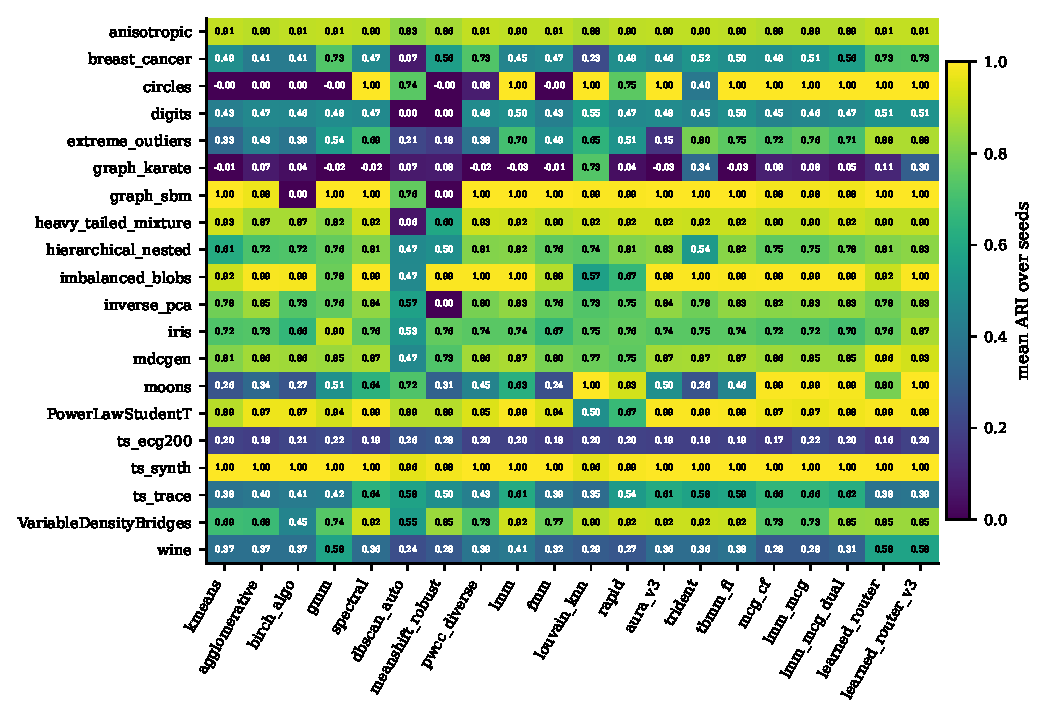
\includegraphics[width=\linewidth]{heatmap.pdf}
  \caption{Mean ARI by dataset family (in-distribution) for classical
  baselines and the new algorithms. \code{louvain\_knn} is the only
  non-router to solve moons and the karate graph together; LMM, spectral
  clustering and AURA-v3 solve circles; GMM is strongest on Iris and Wine.}
  \label{fig:heatmap}
\end{figure}

\subsection{Routers: in-distribution gains, OOD losses}
Figure~\ref{fig:lineage} plots every router generation on both splits.
In-distribution, routers hold the top seven ranks. v2's probe features and
v3's switch from rank voting to per-algorithm ARI regression each added
roughly 0.02--0.03 ARI.
Later architectural changes did not help unless they added a genuinely
different signal. v4 (same features, a different model) overrode v3 on 51 of
52 tasks without improving, so the v5 stacker over $\{$v3, v4$\}$ degenerated
to always-v3. v6's probe signal is different in kind and won exactly one task
v3 missed (inverse-PCA, $0.00 \to 0.38$). That was enough for the v7 stacker
over $\{$v3, v6$\}$ to take rank 1 in round 8. Silhouette as a probe metric
favours compact wrong answers on non-convex data, and adding a 20\% cost term
(v6c) dethroned spectral clustering on close calls where it was correct.

The OOD split reverses the ordering. v3, v5 and v7 make \emph{identical}
picks on every OOD task and lose 0.115--0.126 ARI. v4 loses 0.128. v1 gains
0.023 and v2 loses 0.014. Distance-weighted per-algorithm regressors
extrapolate poorly far from training fingerprints, while v1's rank vote over
neighbours degrades gracefully. Typical OOD failures:
\begin{itemize}
  \item inverse-PCA at $d{=}150$: v3/v7 chose BIRCH (0.27), while RAPID-v3
  scored 0.88.
  \item outlier extremity 10: v3/v7 chose LMM or GMM (0.55), while
  \code{louvain\_knn} scored 0.81.
\end{itemize}
v8 tried to fix this with a richer fingerprint and an OOD-triggered ensemble,
but it regressed by 0.022 against v7 on average. It lost most on the
adversarial regimes it was designed for (\code{VariableDensityBridges}
$-0.092$, \code{PowerLawStudentT} $-0.045$).

\begin{figure}[t]
  \centering
  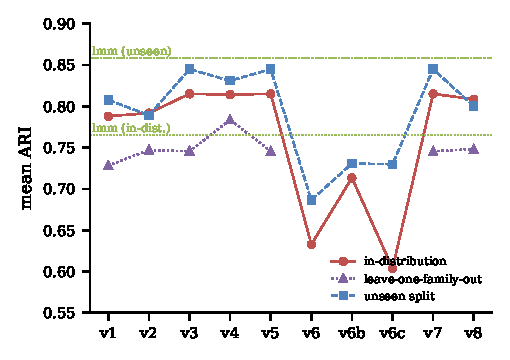
\includegraphics[width=0.55\linewidth]{router_lineage.pdf}
  \caption{Mean ARI of each router generation in-distribution and on the OOD
  split (v8 was not run OOD). LMM is shown for reference. The
  highest in-distribution scorers (v3, v4, v5, v7) show the largest OOD losses.}
  \label{fig:lineage}
\end{figure}

\paragraph{Self-extension.} Routers retrain from the results file, so adding
\code{louvain\_knn} and re-running the benchmark was enough for every
fingerprint router to start dispatching to it on the karate graph. This
raised the mean ARI of v3, v4, v5 and v7 by 0.029--0.038, the largest router
gain since v3, with zero router code changed. Round 15's additions likewise
lifted v7 from 0.871 to 0.912.

\subsection{Machine-proposed algorithms}
The card mutator predicted 0.926 ARI for \code{mutant\_kmeans\_meta}; it
measured 0.747 at introduction and 0.764 in the final snapshot (rank 14). It
beats its parent \code{kmeans\_trimmed} by about 0.05--0.09, so the hybrid is
a real improvement, but the predicted magnitude was not. Bias matching can
order architectures but cannot calibrate them.

Of the round-14 proposals, the two adversarial datasets did what they were
designed to do: routers trailed non-routers by 0.036 and 0.068 ARI on them.
Of the three new algorithms, none reached the top 20.

Trident (rank 10, 0.791) shows the limit of silhouette gating. On moons it
scored 0.265 even though its own \code{louvain\_knn} probe scored 0.997,
because a compact wrong split can have a higher silhouette than a correct
non-convex one.

\subsection{\texorpdfstring{\code{rl\_pipeline}}{rl\_pipeline}}
The behaviour-cloned policy reached 0.59 validation accuracy at predicting the
next action. Chance is 0.125 and the majority-class baseline is 0.41. In a
300-point smoke test it scored ARI 1.00 on blobs and 1.00 on circles, where
$k$-means scores $-0.003$. On circles it chose \code{eigen\_embed} early: from
imitation alone, it learned to switch to the spectral embedding when the cost
stops falling. On moons it scored 0.26, because a $k$-means-like rollout won
the silhouette tie-break.

In the full 43-algorithm benchmark it ranked 36th (mean ARI 0.584), with a
bimodal profile: 0.996 on anisotropic blobs and 0.982 on the SBM graph, but
$-0.001$ on circles at $n{=}500$. At that size the policy still fires
\code{eigen\_embed}, but every rollout then stalls on \code{update\_centers}
no-ops, because 419 imitation rows cannot teach the coordinated sequence that
completes a spectral partition. This is the behaviour-cloning ceiling.
Imitation of per-step decisions does not value a move by where the episode
ends, and compounding errors off the demonstrator distribution are
expected~\cite{ross2011reduction}. In the round-14 sweep, the agent produced
no result rows, which suggests a checkpoint-loading failure in that
configuration that has not yet been resolved.

\section{Lessons}\label{sec:lessons}
\begin{enumerate}
  \item \textbf{Targeted fixes often open new failure modes.} Two of the five
  one-line fixes (\code{dbscan\_auto}, \code{clarans\_pp}) and two of the three
  pipeline v2s (AURA, RAPID) traded the diagnosed failure for a new one. The
  clean pipeline win was META v2, where a brittle rule was strictly replaced.
  \item \textbf{Dispatch pays only when versions are complementary on
  detectable regimes.} AURA-v3 (+0.142) succeeded because effective rank
  separates moons from circles. RAPID-v3 could not help because v2 never won.
  META-v3 lost because its probe was noisier than the v2 it refined.
  \item \textbf{Stacking needs architectural diversity.} Re-fitting the same
  features with a different model (v4) added nothing. A different signal (v6's
  probe) added a real, if small, gain.
  \item \textbf{Learned selection overfits its training distribution, and more
  capacity overfits more.} Only an OOD split shows this. For deployment
  outside the benchmark's distribution, the evidence favours v1, LMM,
  AURA-v2/v3 or \code{louvain\_knn}.
  \item \textbf{Grow the registry, not the router.} The biggest router gains
  came from adding algorithms and data, not from router redesigns.
  \item \textbf{Internal-validity gates are shape-biased.} Silhouette-based
  probes (v6, META-v3, Trident) repeatedly pick compact wrong answers on
  non-convex data. A connectivity-aware criterion or shape prior is needed.
  \item \textbf{Imitation recovers moves, not plans.} The RL agent rediscovered
  \code{eigen\_embed} as a conditional move but not the sequence that makes it
  pay off.
\end{enumerate}

\paragraph{Limitations.} Tasks are small ($n \le 1000$, three seeds), and
lineage tables come from earlier, smaller grids than the final snapshot. The
in-distribution router numbers use task-level leave-one-out with sibling seeds
present. Round-14+ algorithms and GMM were not run OOD. Many ideas here have
prior art: algorithm selection~\cite{rice1976algorithm}, meta-learning for
clustering~\cite{desouto2008ranking,ferrari2015clustering},
landmarking~\cite{pfahringer2000landmarking} (our probe features) and stacked
generalisation~\cite{wolpert1992stacked}. Our contribution is their
systematic, re-runnable evaluation against a broad registry, the
basis-mixture family, and the trajectory-trained agent.

\section{Conclusion and future work}
Starting from benchmark failure modes, we built 25 algorithms and ten
learned selectors and evaluated all of them against one another, including on
data none had seen. The most durable results are a single algorithm (LMM, an
EM-trained mixture over a graph-Laplacian basis) and a negative result (more
sophisticated routers generalise worse). Three directions follow:
\begin{itemize}
  \item fine-tune the behaviour-cloned agent with
  PPO~\cite{schulman2017proximal}, rewarding terminal partition quality, using
  the trajectory corpus every benchmark run now produces;
  \item replace specific weak components, such as CLARANS's swap proposal and
  Chameleon's merge rule, with models trained on trajectory data;
  \item give selection gates a shape-aware criterion, e.g.\ penalise
  silhouette when the number of $k$NN-graph components disagrees with $k$.
\end{itemize}

\paragraph{Availability.} All algorithms, configurations, results and the
figure scripts are at \url{https://github.com/Ashail33/clustbench}.

\bibliographystyle{unsrtnat}
\bibliography{../references}

\end{document}
